\documentclass[11pt]{article}

\usepackage{geometry}
\geometry{margin = 1in,top =0.12\paperheight, headheight=\paperheight}
\usepackage[export]{adjustbox}
\usepackage{array}
\usepackage{amsmath}
\usepackage{amsfonts}
\usepackage{fancyhdr}
\usepackage{lastpage}
\usepackage{xcolor}
\pagestyle{fancy}
\fancyhf{}
\rhead{Written Assignment, Page \thepage}
\lhead{MATH211}
\chead{
\includegraphics[width = 0.15\textwidth]{MCLogo-Bck.png}}


%\renewcommand{\footrulewidth}{0.4pt}

\usepackage{enumitem}
\usepackage{pifont}
\usepackage{graphicx}
\graphicspath{{../img}}

\newtheorem{theorem}{Theorem}
\newtheorem{exercise}{Exercise}


\newcommand{\R}{\mathbb R}
\newcommand{\e}{{\rm e}}
\newcommand{\inpr}[1]{\left\langle#1\right\rangle}
\newcommand{\norm}[1]{\lVert #1 \rVert}
\newcommand{\abs}[1]{\lvert #1 \rvert}
\newcommand{\vv}{\mathbf v}
\newcommand{\uv}{\mathbf u}

\DeclareMathOperator{\xd}{d\!}
\DeclareMathOperator{\proj}{proj}

\title{}
\date{}

\begin{document}
\noindent {\bf Problems.} 
\begin{enumerate}
\item
Suppose $\mathbf u$ and $\mathbf v$ are two nonzero vectors configured as in the following figure:
\begin{figure}[h]
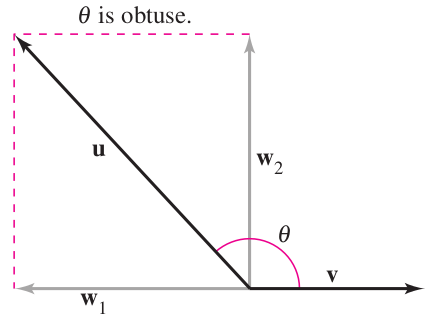
\includegraphics[width = .25\textwidth, center]{proj2.png}
\end{figure}

Prove that 
\begin{equation*}
\label{vecproj}
\proj_{\mathbf v}\mathbf u = \left(\frac{\mathbf v\cdot\mathbf u}{\norm{\mathbf v}^2}\right)\mathbf v
\end{equation*}

\vspace{\stretch{2}}
\item
Use the dot product to verify that $\mathbf u- \proj_{\mathbf v}\mathbf u $ is orthogonal to $\mathbf v$. (Recall that two non-zero vectors are orthogonal if and only their dot product equals zero.)
\vspace{\stretch{1}}
\end{enumerate}


\end{document}